\part{MaterialApp}

\section{Struktur program}

Berikut ini adalah struktur program sederhana yang akan digunakan
\begin{dartcode}
import 'package:flutter/material.dart';
  
void main() => runApp(MyApp());
  
class MyApp extends StatelessWidget {
  @override
  Widget build(BuildContext context) {
    return MaterialApp(
      title: 'Flutter Demo',
      theme: ThemeData(
        primarySwatch: Colors.blue,
      ),
      home: MyHome(),
    );
  }
}
  
class MyHome extends StatelessWidget {
  @override
  Widget build(BuildContext context) {
    return Scaffold(
      appBar: AppBar(
        title: Text('MyHome')
      ),
      body: Center(
        child: Text('This is my home'),
      ),
    );
  }
}
\end{dartcode}

Tampilan dari program ini dapat dilihat pada Gambar \ref{fig:MyHome-debug}.
\begin{marginfigure}
{\centering
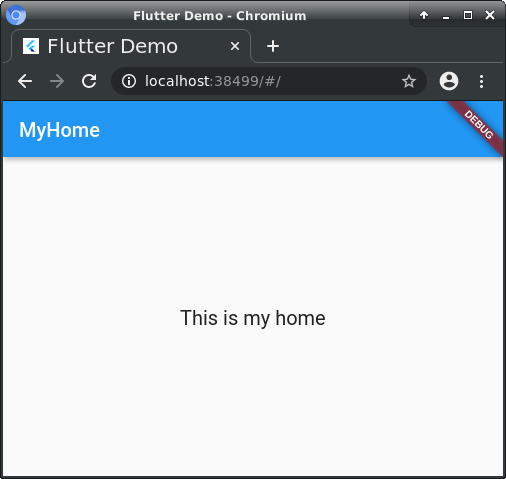
\includegraphics[width=\marginparwidth]{images/MyHome_debug.png}
\par}
\caption{Tampilan MyHome.}
\label{fig:MyHome-debug}
\end{marginfigure}

\section{Menghilangkan banner debug}

Banner debug pada tampilan aplikasi dapat dihilangkan dengan
mengatur parameter \\
\txtinline{debugShowCheckedModeBanner} menjadi \txtinline{false}.

Contoh:
\begin{dartcode}
class MyApp extends StatelessWidget {
  @override
  Widget build(BuildContext context) {
    return MaterialApp(
      title: 'Flutter Demo',
      theme: ThemeData(
        primarySwatch: Colors.blue,
      ),
      home: MyHome(),
      debugShowCheckedModeBanner: false,
    );
  }
}
\end{dartcode}

\begin{marginfigure}
{\centering
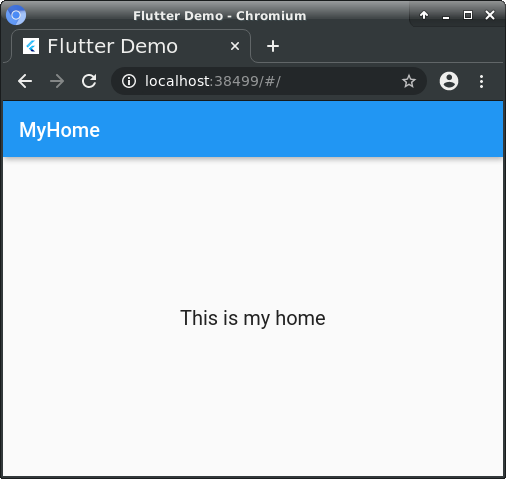
\includegraphics[width=\marginparwidth]{images/MyHome_01.png}
\par}
\caption{Tampilan MyHome tanpa banner debug.}
\end{marginfigure}